\chapter{\xlabel{tweak}Tailoring Your Reduction}
\label{sec:tweak}


\section{Adding and amending parameters}
The configuration file \file{dimmconfig\_jsa\_generic.lis} is a good
configuration file to use as a first pass for reducing any data, and is
the default configuration used by the pipeline's \drrecipe{REDUCE\_SCAN}
recipe.

\textbf{You can create your own personalised configuration file from
scratch or copy one of the provided ones to your local directory and
edit it.}

The first line of each specialised configuration file is often the path
to another configuration file --- known as the \emph{parent} configuration
file. The new configuration file inherits all the parameter values
defined by the parent configuration file, and then goes on to specify
additional parameter settings which may supplement or over-ride those
defined in the parent configuration file. Parameters that are not set to
a specific value by \emph{either} configuration file assume the default
values listed in \cref{Appendix}{app:parameters}{Configuration-parameter
descriptions}\footnote{These default values are defined in the file
\texttt{\$SMURF\_DIR/smurf\_makemap.def}.}.

Often you will want to use one of the pre-defined configuration files
included within \starlink\ tree as the parent configuration. Remember
that any parameters appearing in your configuration file
automatically override the values supplied by the parent file. As an
example, consider the following text file ``\texttt{myconf}'':

\begin{terminalv}
% cat myconf

#  This is an example configuration file.
^$STARLINK_DIR/share/smurf/dimmconfig_jsa_generic.lis

numiter=-100
maptol=0.01

\end{terminalv}

The first thing to note is that blank lines and comment lines
(\emph{i.e.} lines beginning with the hash character ``\texttt{\#}'') are
ignored and can be used to document your configuration file. Next note
that this example file uses
\texttt{\$STARLINK\_DIR/share/smurf/dimmconfig\_jsa\_generic.lis} as its
parent (the path to the parent file must be preceded
by an up-caret (\texttt{\^}) character). Thus, all the parameter values
set by \texttt{\$STARLINK\_DIR/share/smurf/dimmconfig\_jsa\_generic.lis} are
first read, before adding in other parameter settings. In this case, values
are assigned to \param{maptol} and \param{numiter}, over-riding the
values provided by the parent file.

You can use more than one parent file if required (each one a separate
line, and preceded by an up-caret). Each specified parent will be read in
turn, with parameter settings read from later ones having priority over
those read from earlier ones.

You can also add or amend parameters by listing them directly on the
command line. They are appended to the configuration file name as a
comma separated list as shown in the example below. Be sure to include
all the necessary quotation marks.

\begin{terminalv}
% makemap in='s8*.sdf' out=850map \
       config='"^dimmconfig\_jsa\_generic.lis,numiter=-50,exportndf=(flt,noi),itermap=1"'
\end{terminalv}

For full details of all the possible ways of specifying groups of
parameter values, see Section ``\xref{Specifying Groups of
Objects}{sun95}{se_groups}'' in ``\xref{Starlink User Note 95}{sun95}{}.

\textbf{What parameters can be changed?}\\*
\cref{Appendix}{app:parameters}{Configuration-parameter descriptions}
lists the parameters that are more likely to be of interest to you when
creating your own configuration files. You can also change any of the
other more esoteric parameters not included in that list --- see
Appendix \xref{SUN/258} {sun258}{par_full} within \xref{Starlink
User Note 258}{sun258}{} for a full list -- but we do not advise this.

\begin{tip}
  If some feature is switched on either by default or within
  the parent configuration file, it can be switched off if required
  by assigning a suitable value to the corresponding parameter within
  your own configuration file. The value needed to do this will be
  given in the parameter description in \cref{Appendix}{app:parameters}
  {Configuration-parameter descriptions} --- for instance it may be
  \param{<undef>}, or \param{0}, or some other special value.
\end{tip}

\textbf{Note:} any parameter can be made wavelength dependent by
adding the prefix \param{450.} or \param{850.}, e.g.
\param{flt\_edge\_largescale} applies to both 450\,$\mu$m and
850\,$\mu$m whilst \param{450.flt\_edge\_largescale} applies to
450\,$\mu$m only. Be aware that if both are specified, unqualified
values (no prefix) take priority over qualified values.

\section{\xlabel{inter}Writing out models \& intermediate maps}
\label{sec:inter}

\textbf{itermaps}\\
Setting the parameter \setparam{ITERMAP}{itermap}{1} writes out the
map containing the astronomical signal after each iteration. Setting
\param{itermap~=~2} adds the QUALITY component.  These can be visually
inspected with

\begin{terminalv}
% gaia 850map.more.smurf.itermaps
\end{terminalv}

to help determine an appropriate number of iterations. Alternatively, you
can view several itermaps simultaneously side-by-side (\emph{e.g.}
\cref{Figure}{fig:itermaps}{Initial six itermaps}) using \Kappa\ as
described in \cref{Section}{sec:itermaps}{Monitoring the map at the
end of each iteration}.

Viewing itermaps is useful when a fixed number of iterations have been requested (i.e. a positive
value for \xparam{NUMITER}{numiter}) and the map solution diverges before
they have completed. See also \cref{Section}{sec:itermaps}{Monitoring the map
at the end of each iteration} for how to view these maps whilst \makemap\ is still running.
\newline\newline
\textbf{shortmaps}\\
If the parameter \param{shortmaps} is non-zero, a map is made from
every group of adjacent time-slices (as specified by the parameter).
These are stored as an NDF extension and can be viewed \gaia.

\begin{figure}[ht!]
\begin{center}
\begin{fmpage}{0.95\linewidth}
\vspace{0.2cm}
\hspace{2mm}
\textbf{Viewing ITERMAPs}
\minipageclear
\vspace{0.5cm}

\begin{minipage}[c]{0.65\linewidth}

\begin{terminalv}
% stackframes map.more.smurf.itermaps \
sort=false map_itermaps
\end{terminalv}
\end{minipage}
\hspace{0.3cm}
\begin{minipage}[c]{0.29\linewidth}
Stack the individual itermaps into a single cube (\textsc{Kappa}
\xref{PASTE}{sun95}{paste} can also be used).
\end{minipage}
\minipageclear

\vspace{0.5cm}

\begin{minipage}[c]{0.65\linewidth}
\centering
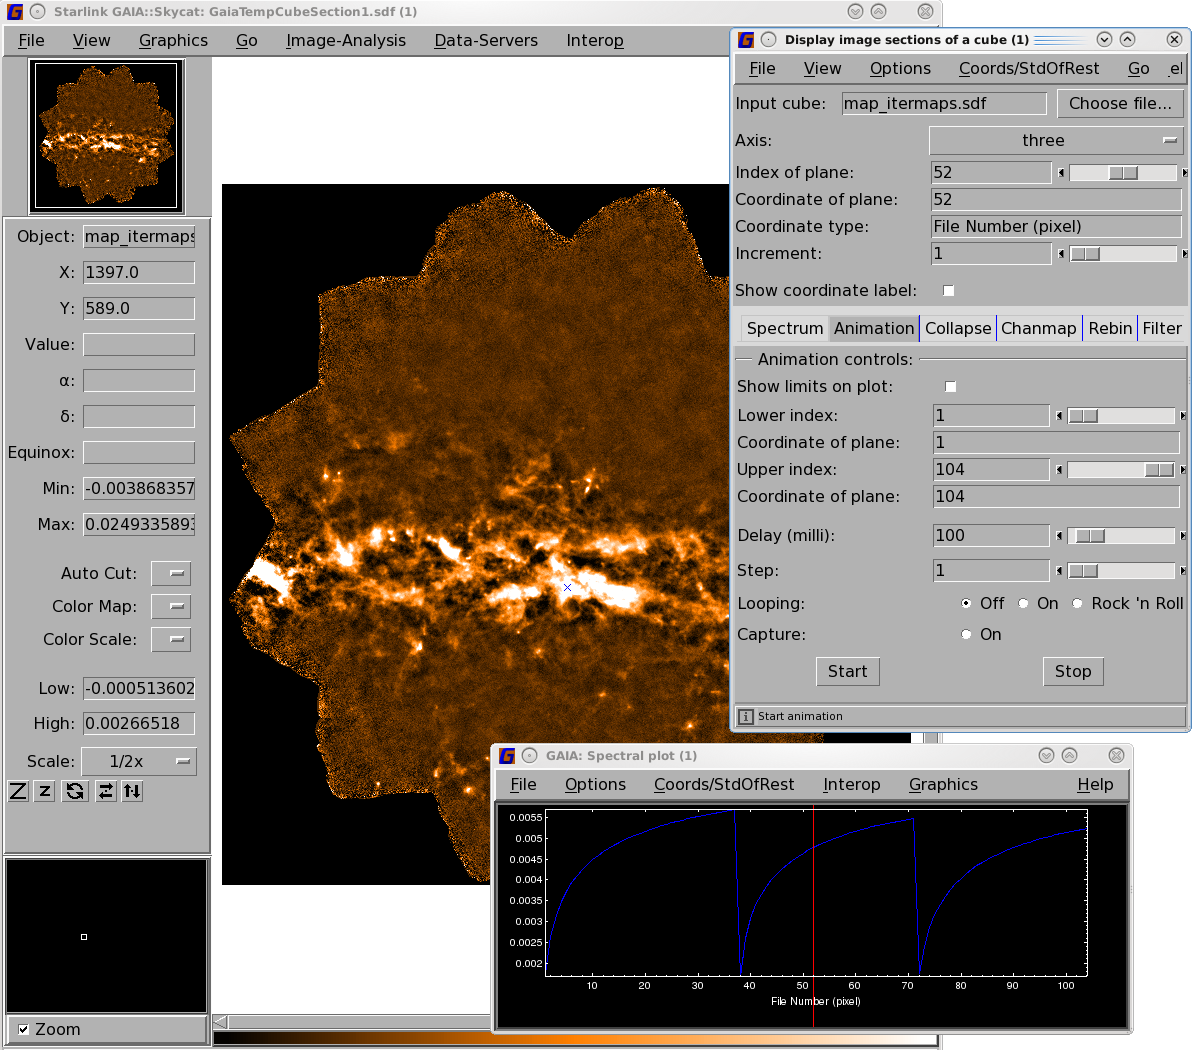
\includegraphics[width=0.95\textwidth]{sc21_itermaps_anim}
\end{minipage}
\hspace{0.3cm}
\begin{minipage}[c]{0.29\linewidth}
The output map \file{map\_itermaps} can be opened with \gaia. The data used
in this example is the Galactic map reduced in
\cref{Section}{sec:bright_ex}{\file{dimmconfig\_bright\_extended.lis}}. The
Spectral plot window shows the value for a single pixel and the three
chunks are easily identified. You can select the \gaiathing{Animation} tab
in the \gaiathing{Display image sections} window and click
\gaiathing{Start} to loop through the itermaps for each iteration.  The
`movie' will appear in the main \gaia\ window.
\end{minipage}
\minipageclear

\vspace{0.7cm}

\begin{minipage}[c]{0.65\linewidth}
\centering
\hspace{0.5mm}
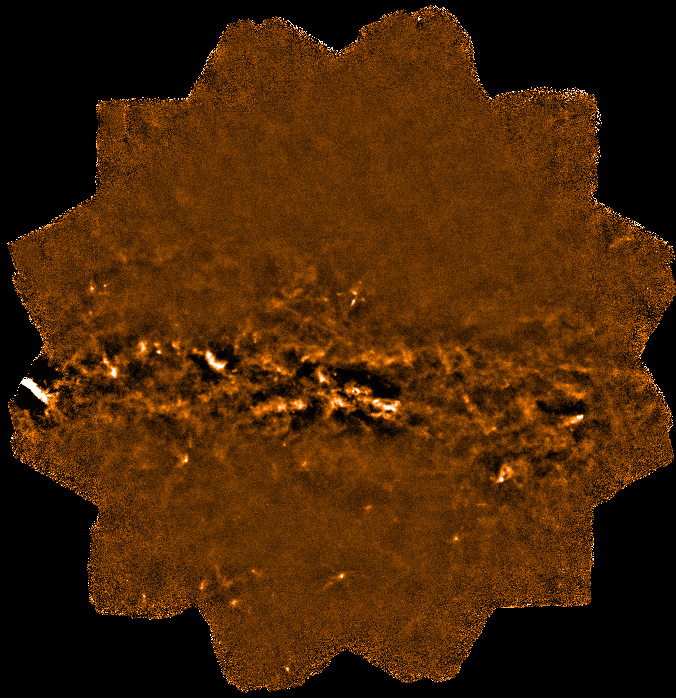
\includegraphics[width=3cm, ]{sc21_iter1}
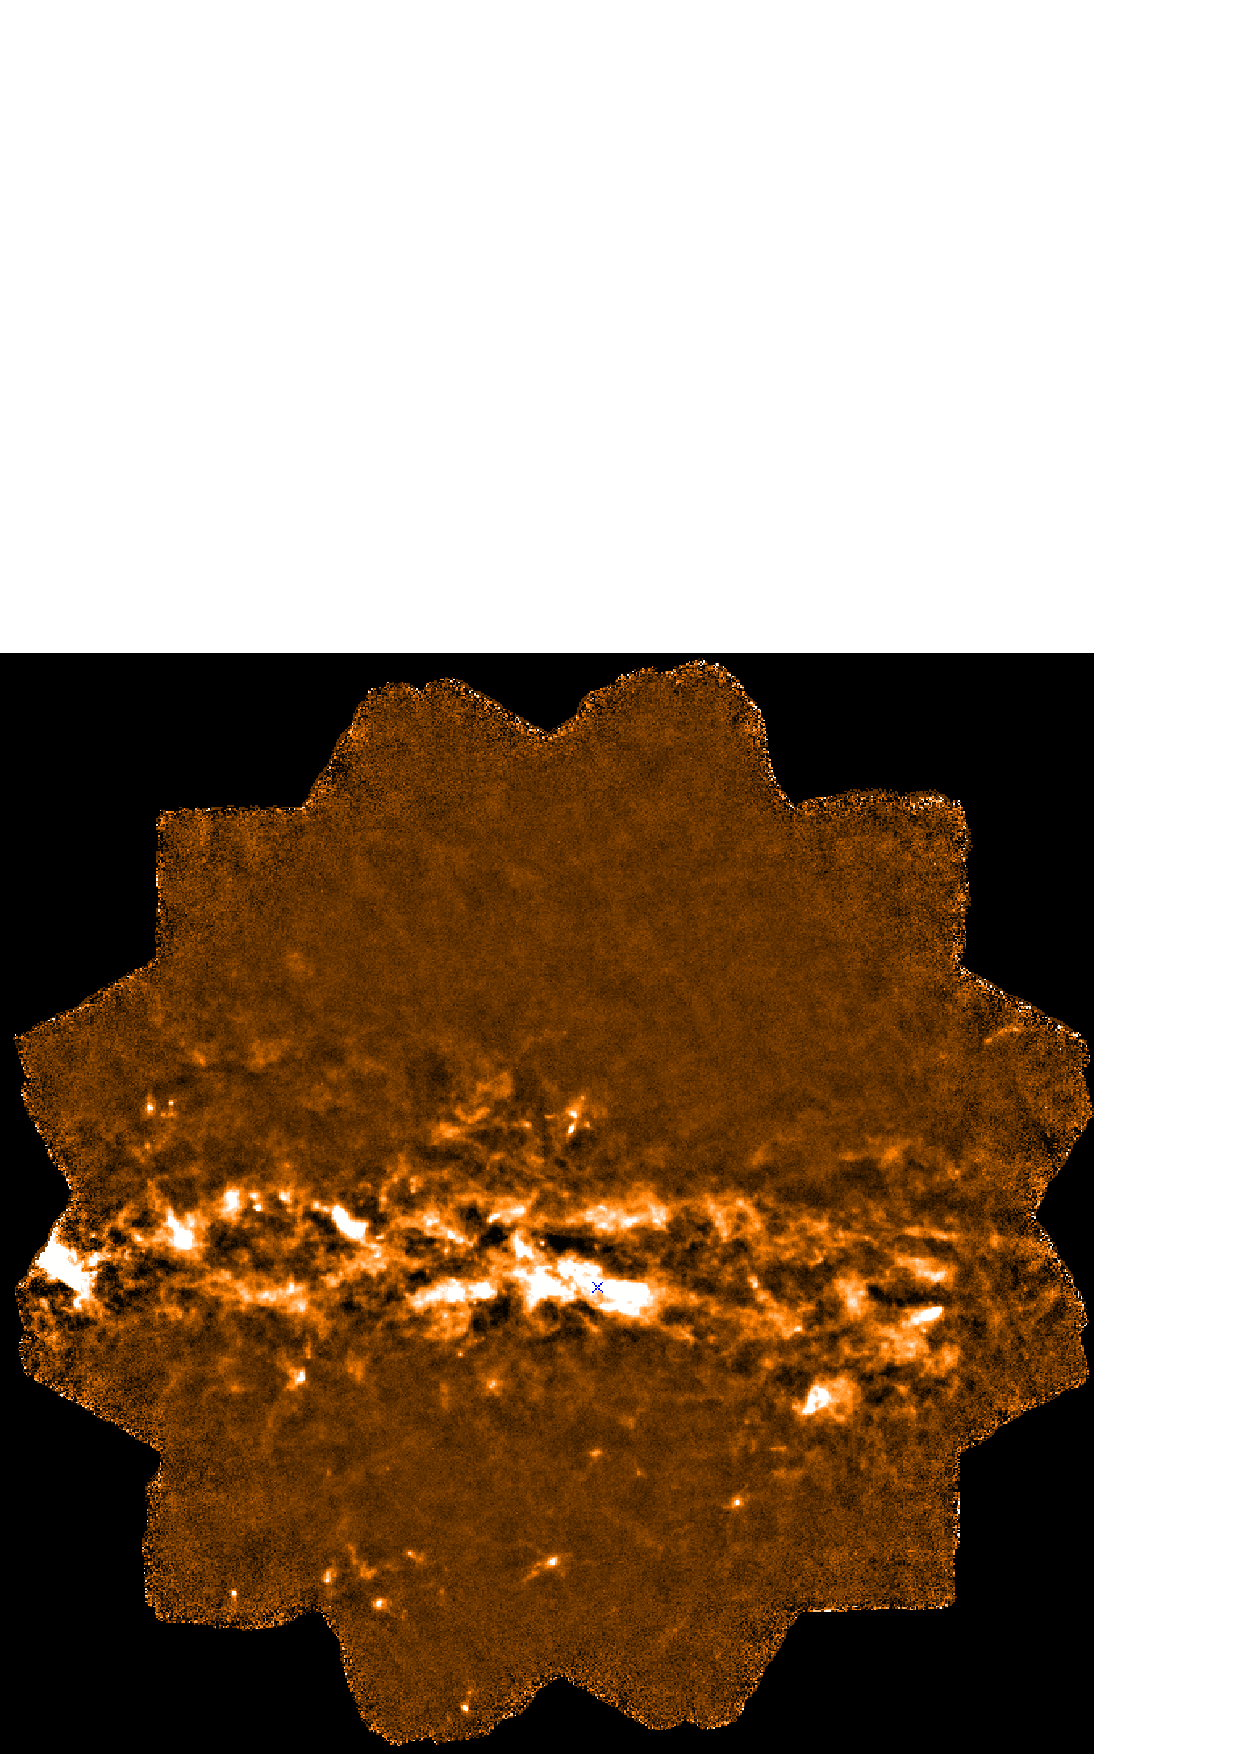
\includegraphics[width=3cm, ]{sc21_iter2}
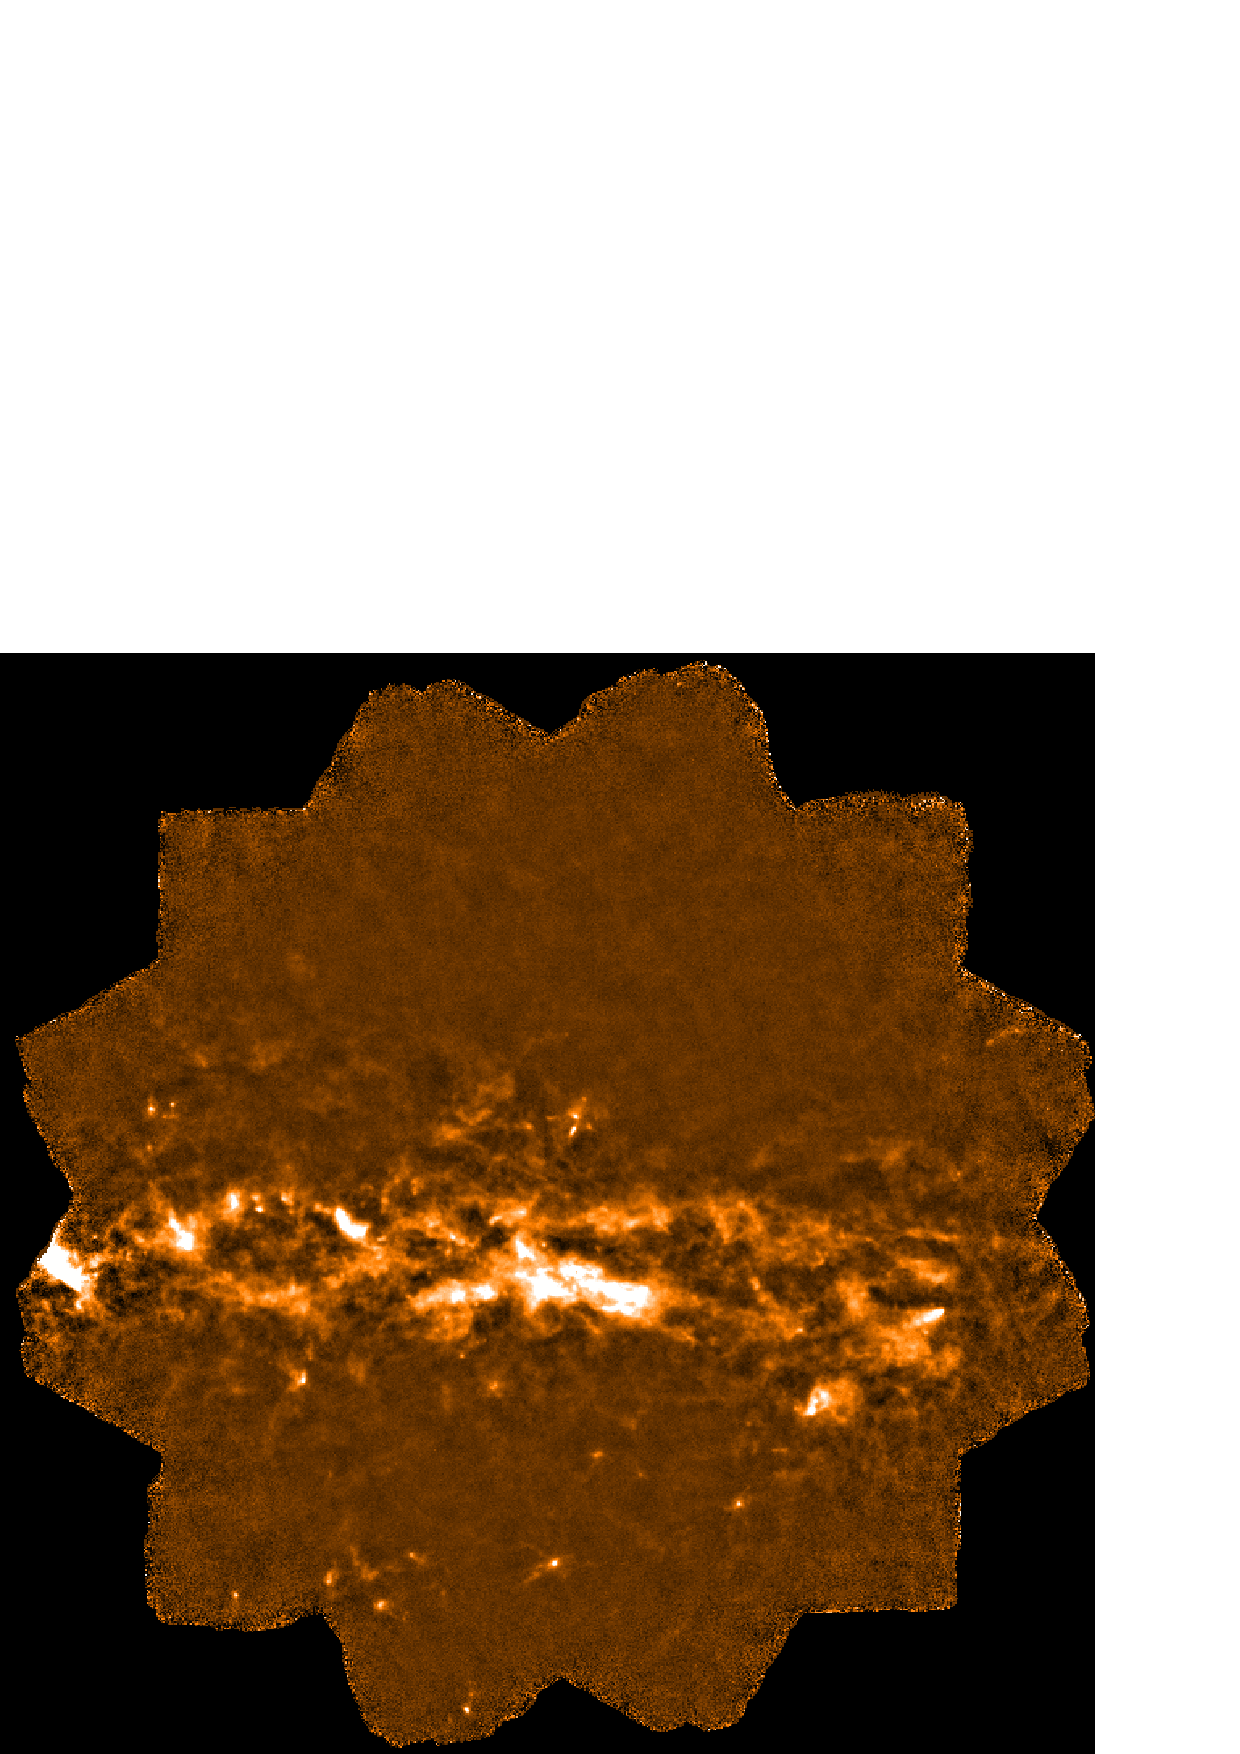
\includegraphics[width=3cm, ]{sc21_iter31}
\vspace{0.2cm}
\end{minipage}
\hspace{0.3cm}
\begin{minipage}[c]{0.29\linewidth}
These windows show the itermaps map at 1, 10, and 30 iterations. A
specific iteration can be selected using the \gaiathing{Index of plane}
slider on the \gaiathing{Display image sections} window.
\vspace{0.2cm}
\end{minipage}
\minipageclear
\end{fmpage}
\end{center}
\caption[View maps for each iteration]{
  \small Example using the \smurf\ command \stackframes\ and
  \gaia\ to view the `itermap' for each iteration.
}
\label{fig:stack}
\end{figure}


\begin{terminalv}
% gaia 850map.more.smurf.shortmaps
\end{terminalv}

You can view the shortmaps and itermaps more
conveniently by stacking them into a single cube using the \smurf\
command \stackframes. This cube can then be viewed as a
`movie' with \gaia, using the animation option to loop through the
itermaps. See \cref{Figure}{fig:stack}{the box above} for instructions.
\newline\newline
\textbf{exportmodel}\\
This parameter has been discussed in
\cref{Section}{sec:export}{Exporting individual models} and allowed
you to see the model that was fit for each component specified by the
\xparam{MODELORDER}{modelorder} parameter.

\section{\xlabel{filt}Large-scale filtering}
\label{sec:filt}

Some of the most important parameters to experiment with are the
filtering options. By default, no filtering is applied during the
pre-processing stage\footnote{However, the \blankfield\ configuration
over-rides this default.} (see \xparam{FILT_EDGE_LARGESCALE}{filt\_edge\_largescale}
and \xparam{FILT_EDGE_SMALLSCALE}{filt\_edge\_smallscale}). A high-pass
filter is used during the iterative stage if \xparam{MODELORDER}{moelorder}
includes \model{FLT}\footnote{The \blankfield\ configuration omits
\model{FLT} from \param{modelorder}.}, and selected a suitable value
for the filter size is crucial for maps containing extended emission.

The maximum spatial scale of structure that can be recovered by the
map-maker is determined by the scanning speed and frequency cut
applied to the data:

\begin{equation}
\frac{\textrm{speed}[arcsec / \textrm{s}]}{\textrm{frequency
    cut}[\textrm{Hz}]}=\textrm{scale size}[arcsec]
\end{equation}

The default (\emph{i.e.} if no configuration is supplied) filter sizes
in arc-seconds are:

\setparam{FLT.FILT_EDGE_LARGESCALE}{450.flt.filt\_edge\_largescale}{200} \\
\setparam{FLT.FILT_EDGE_LARGESCALE}{850.flt.filt\_edge\_largescale}{480}.

To make your life easier, these parameters allow you to specify the
filter limits in terms of spatial scale in arc-seconds---in this case
480\,arcsec at 850\,$\mu$m and 200\,arcsec at 450\,$\mu$m. For example,
at 850\,$\mu$m, recovering scales of 480\,arcsec at a scan speed of
600\,arcsec/sec (default for a 1 degree \textsc{pong}) corresponds to
a frequency of 1.25\,Hz.

Choosing a high-pass filter is especially important for the recovery
of extended emission. The \brightextended\ configuration file sets
\setparam{FLT.FILT_EDGE_LARGESCALE}{flt.filt\_edge\_largescale}{480}
for both 450\,$\mu$m and 850\,$\mu$m. Be aware that increasing filter sizes
decreases the flatness of your background. A compromise must be made between
extended structure and the flatness of your map. See \cref{Figure}{fig:fltcompare}
{the figure below} for an illustration of the effect of
\xparam{FLT.FILT_EDGE_LARGESCALE}{flt.filt\_edge\_largescale} on your map.

The scanning speeds are fixed for a given observing mode; you can find
out the speed at which your data were taken from the
\texttt{SCAN\_VEL} keyword in the FITS header (see
\cref{Section}{sec:fitsheader}{Headers and file structure}).

%\pagebreak[4]
\textbf{Flattening the background}\\*
There is an option to reduce the noise in your background introduced by
setting a high value for the large-scale filter. The parameter
\xparam{FLT.FILT_EDGE_LARGESCALE_LAST}{flt.filt\_edge\_largescale\_last}
filters the regions outside your \model{AST} mask (see \cref{Section}
{sec:astmask}{AST masking}) on a shorter scale for the last iteration only,
thereby producing a much flatter background. Note that this is probably a
bad idea if you intend to co-add several observations, as it removes
potentially real structure in the background regions that could otherwise be
recovered by co-adding several observations. In general, use of
\param{flt.filt\_edge\_largescale\_last} should be seen as a cosmetic
enhancement, since it results in differing filter sizes being used inside
and outside the \model{AST} mask.

Also note that when using \param{flt.filt\_edge\_largescale\_last} the
variances stored in the final map are from the penultimate iteration in
order to avoid using the artificially reduced variances created on the
last iteration.

\begin{figure}
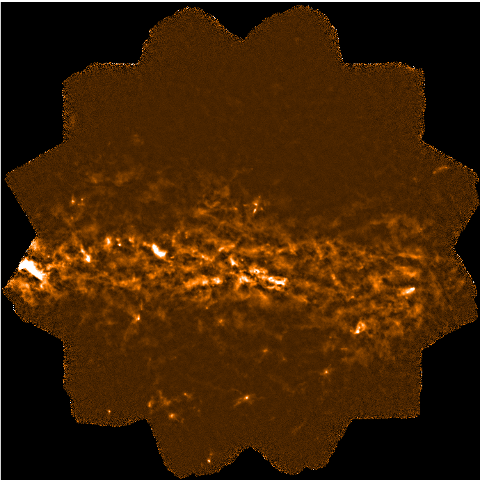
\includegraphics[width=0.46\linewidth]{sc21_brex_19}
\hspace{7mm}
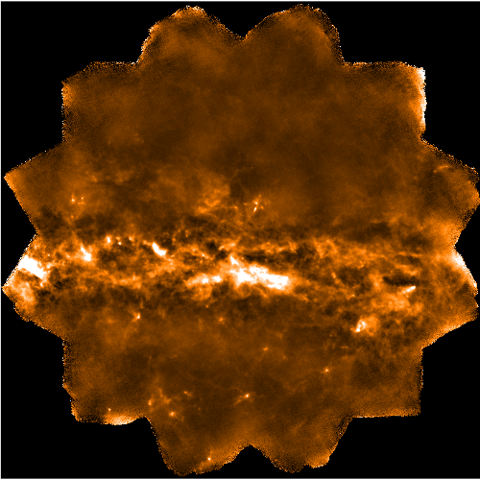
\includegraphics[width=0.46\linewidth]{sc21_brex_18}
\caption[Illustrating the effects of high-pass filtering]{
  Highlighting the effects of high-pass filtering on your map.
  \textbf{(Left)} Map made with \param{850.flt.filt\_edge\_largescale}{300}.
  \textbf{(Right)} Map made with \param{850.flt.filt\_edge\_largescale}{1000}.
  All other configuration parameters remain the same.\label{fig:fltcompare}
}
\end{figure}


\section{\xlabel{fitcom}Fitting COM for each sub-array}
\label{sec:fitcom}

A useful option to improve the flatness of your maps is to fit the
\model{COM} model independently for each sub-array. This is
particularly effective if you find you have one sub-array noisier than
the others.

This comes with the warning however that you will lose information on
any scales larger than the area covered by a single sub-array. It is
therefore not recommended if you have very large-scale extended
structure.

To initialise this option set \setparam{COM.PERARRAY}{com.perarray}{1}.


\section{\xlabel{noibox}Flagging bad data}
\label{sec:noibox}

Bolometers that have higher noise levels are down-weighted when forming
the map. By default, a separate noise estimate is created for each
15 second section\footnote{15 seconds is half a sub-scan.} of each bolometer
time-stream, but an alternative length can be specified using parameter
\xparam{NOI.BOX_SIZE}{noi.box\_size}.

Dividing each bolometer up into sections helps to remove `scuffs' or other
noise artefacts you might see in your error map due to a sub-array (or
arrays) temporarily jumping to a higher noise state. As the section length
tends to 1 second we find some of the source signal being down-weighted.
Higher than this 15 seconds and the map-maker becomes less sensitive to
the higher noise states.

Other parameters you may want to try include \xparam{FLAGFAST}{flagfast} and
\xparam{FLAGSLOW}{flagslow}. You may find that setting \param{flagfast} to less
than the default of 1000\,arcsec/sec will help reduce the effect of any
`smearing' of sources (and of noise) in maps, while setting
\param{flagslow} greater than the default of 300\,arcsec/sec helps to
flatten the edges of maps. To determine reasonable values for your
 data-set you should do \jcmtstate\ and view the scan speed using
\topcat. See \cref{Section}{sec:scan}{Displaying scan patterns} for
details.


\section{\xlabel{maskbe}Using external masks}
\label{sec:maskbe}

For an introduction to the purpose and effects of masking, see
\cref{Section}{sec:masking}{Masking}.

As an S/N mask is redetermined after each iteration it changes with the map
 which can sometimes cause convergence problems. The mask
will also depend on the amount of data going into the map and the
pixel size. A fixed externally supplied mask  can get around these problems.

The sequence below is a summary of the procedure for generating and
supplying an external mask. In this example the mask is generated from
the map produced by an initial run through the map-maker.
Alternatively maps from other observatories can be used.

These steps are followed in the example in
\cref{Section}{sec:bright_ex}{Extended galactic sources}.

\begin{aligndesc}
\item[Step~1] Generate a map covering your region. This may be by
  simply running the map-maker on your data as shown below.
\begin{terminalv}
% makemap in='s8*.sdf' out=850map \
          config='"^dimmconfig_bright_extended.lis"'
\end{terminalv}
The alternative is to access a map from a different data-set or even a
different telescope, e.g. a map downloaded from the Herschel Science
Archive. For instructions on converting from FITS to NDF see
\cref{Appendix}{app:fits}{Convert format from FITS to NDF}.\\

\item[Step 2] Make a signal-to-noise map using the \Kappa\ command
  \makesnr.
\begin{terminalv}
% makesnr 850map 850map_snr
\end{terminalv}

\item[Step 3] Threshold this S/N map to set everything below
  3$\sigma$ to 0 and everything above to 1.
\begin{terminalv}
% thresh 850map_snr 850map_mask thrlo=3 newlo=0 thrhi=3 newhi=1
\end{terminalv}
This generates a mask which has an unrealistic hard 3$\sigma$
cut-off. Step 4 is performed to smooth the the edges of your mask.

\item[Step 4] Smooth the thresholded map with a Gaussian filter
  of FWHM of 5 pixels (=\,20\,arcsec). Then it is again thresholded,
  this time keeping everything above 5\,\% of the 0 level as the mask
  and setting the rest to \texttt{bad}.
\begin{terminalv}
% gausmooth 850map_mask 850map_mask_sm fwhm=5
% thresh 850map_mask_sm 850map_mask_zm thrlo=0.05 newlo=bad \
  thrhi=0.05 newhi=1
\end{terminalv}

\item[Step 5] Finally the map is re-made with this mask supplied as an
  external file. Notice that the extra parameters required to pick up
  this external mask are being appended to the configuration file on
  the command line rather than editing the file itself.
\begin{terminalv}
% makemap in='s8*.sdf' out=850map_zm ref=850map_mask_zm \
          config='"^dimmconfig_bright_extended.lis,ast.zero_mask=1,\
                   ast.zero_snr=0"'
\end{terminalv}

\end{aligndesc}

\section{\xlabel{skyloop}Skyloop}
\label{sec:skyloop}

\starfig{sc21_skyloop}{}{width=0.55\linewidth}{fig:skyloop}{
  Illustration of the \task{skyloop} approach}{
  Illustration of the \task{skyloop} approach
  to map-making compared with the standard map-maker.
}

Traditionally, the map-maker divides a non-contiguous sequence of time
series data into chunks. It processes each chuck independently
before co-adding them as a final step in the the reduction---see
\cref{Figure}{fig:skyloop}{the figure below}.

This means for each chunk the map-maker has to start from scratch
determining the \model{AST} model, and the benefit of long integration
times spent building up the signal is lost. Configuration files that use
signal-to-noise masks especially suffer from this approach as the
signal-to-noise in each individual chunk can remain low and fainter
extended structure is not recovered.

The \skyloop\ command is a script that runs \makemap\ multiple times
performing just a single iteration on each occasion. It starts by
performing a single iteration of \task{makemap} from which a
co-added map is generated. This map is then supplied as an initial
estimate of the sky for the next invocation of \task{makemap}. On
this next invocation, the initial sky estimate is subtracted from the
cleaned time-series data and the \model{COM}, \model{GAI},
\model{FLT}, \model{EXT} models are subtracted. This produces a new
model of the sky (from the current iteration) to which the sky
estimate (from the previous iteration) is then added. In this way the
signal from all of the chunks is built up over the iterations and is
all included in the final map estimate when convergence is reached.




Be aware that \task{skyloop} uses a lot of disk space. Setting
environment variable \envvar{STAR\_TEMP} to a suitable location
before you start will prevent \task{skyloop} from crashing
if you run out of temporary storage space.
\begin{terminalv}
% setenv STAR_TEMP /some/directory/with/a/lot/of/space
\end{terminalv}
\task{skyloop} can then be called in a way very similar to \makemap, with
a configuration file specified on the command line.
\begin{terminalv}
% skyloop in=^myfiles.lis out=map_skyloop config=^dimmconfig_bright_extended.lis
\end{terminalv}

\section{Troubleshooting}

\begin{table}[b]
\begin{center}
\begin{tabular}{|p{5cm}|p{10.5cm}|}
\hline
\textbf{PROBLEM} & \textbf{POSSIBLE SOLUTION}\\
\hline
I have blobs in my map that look like big thumbprints. & Try adding
\fixblobs\ into your configuration file (see \cref{Section}{sec:problem}
{Configuration files for solving specific problems}).  Note that this sets
\setparam{COM.SIG_LIMIT}{com.sig\_limit}{5} which is somewhat
conservative. You can experiment by lowering this, but we would not recommend
lower than $\sim$2 because you may then lose too many samples.

In addition, check you are not using \setparam{FLT.NOTFIRST}{flt.notfirst}{1} as this
can make blobs worse.\\
\hline
I want to recover more extended structure. & There is a trade off
between extended emission and noise in your map. If you are willing to
accept more low frequency noise you can increase the filter scale with
\xparam{FLT.FILT_EDGE_LARGESCALE}{flt.filt\_edge\_largescale}. The default is 480\,arcsec but you
could try 600\,arcsec. To reduce the increased background noise you can set
\setparam{FLT.FILT_EDGE_LARGESCALE_LAST}{flt.filt\_edge\_largescale\_last}{200}. This
sets the background filtering to 200\,arcsec for the final iteration
only, though you can go as low as you want with it. Note, this should be
seen as a mainly cosmetic effect as it causes the map to use different
filter sizes in different regions, making interpretation of the map difficult. \\
\hline
I want a flatter background.  & Try \setparam{COM.PERARRAY}{com.perarray}{1}, although
be aware this will lose structure on scales larger than a sub-array.
If you are chasing extended emission see the point above. For a more uniform
background set \xparam{FLT.FILT_EDGE_LARGESCALE_LAST}{flt.filt\_edge\_largescale\_last}
to a small value to get harsh filtering on your final iteration.\\
\hline
I have linear striations in my map making my background look
scratchy.& Try setting \setparam{COM.CORR_ABSTOL}{com.corr\_abstol}{0.8} [default=0.2].
This rejects more bolometers with deviant common-mode signals.
However, as more bolometers are removed there are fewer data available
for your final map, resulting in higher noise.\\
\hline
My map will not converge. & Try adding \fixconvergence\ into your
configuration file (see \cref{Section}{sec:problem}{Configuration files
for solving specific problems}).  This prevents the masks from changing
after ten iterations.\\
\hline
\end{tabular}
\end{center}
\end{table}







